Se midieron los patrones de difracción de la sal de mesa y la sal \textit{light}, así como también de las soluciones de cloruro de potasio y bromuro de potasio, de estas sales en estado puro y de una mezcla de ambas.

poner aca la sal de mesa y sal light

En las mediciones de las soluciones de KCl y KBr, variando la fracción molar $X_{Br}$ en valores de 0, 0.2, 0.4, 0.6, 0.8 y 1, se observó un desplazamiento progresivo en los picos de intensidad. Inicialmente, los patrones presentan una mayor similitud con el KCl puro, evolucionando gradualmente hacia el perfil del KBr conforme aumenta la concentración de bromo. Este fenómeno se ilustra en la figura \ref{fig:zoom_picos}, donde se aprecia el desplazamiento de los picos de mayor intensidad para cada una de las soluciones analizadas.


\begin{figure}[htbp]
    \centering
    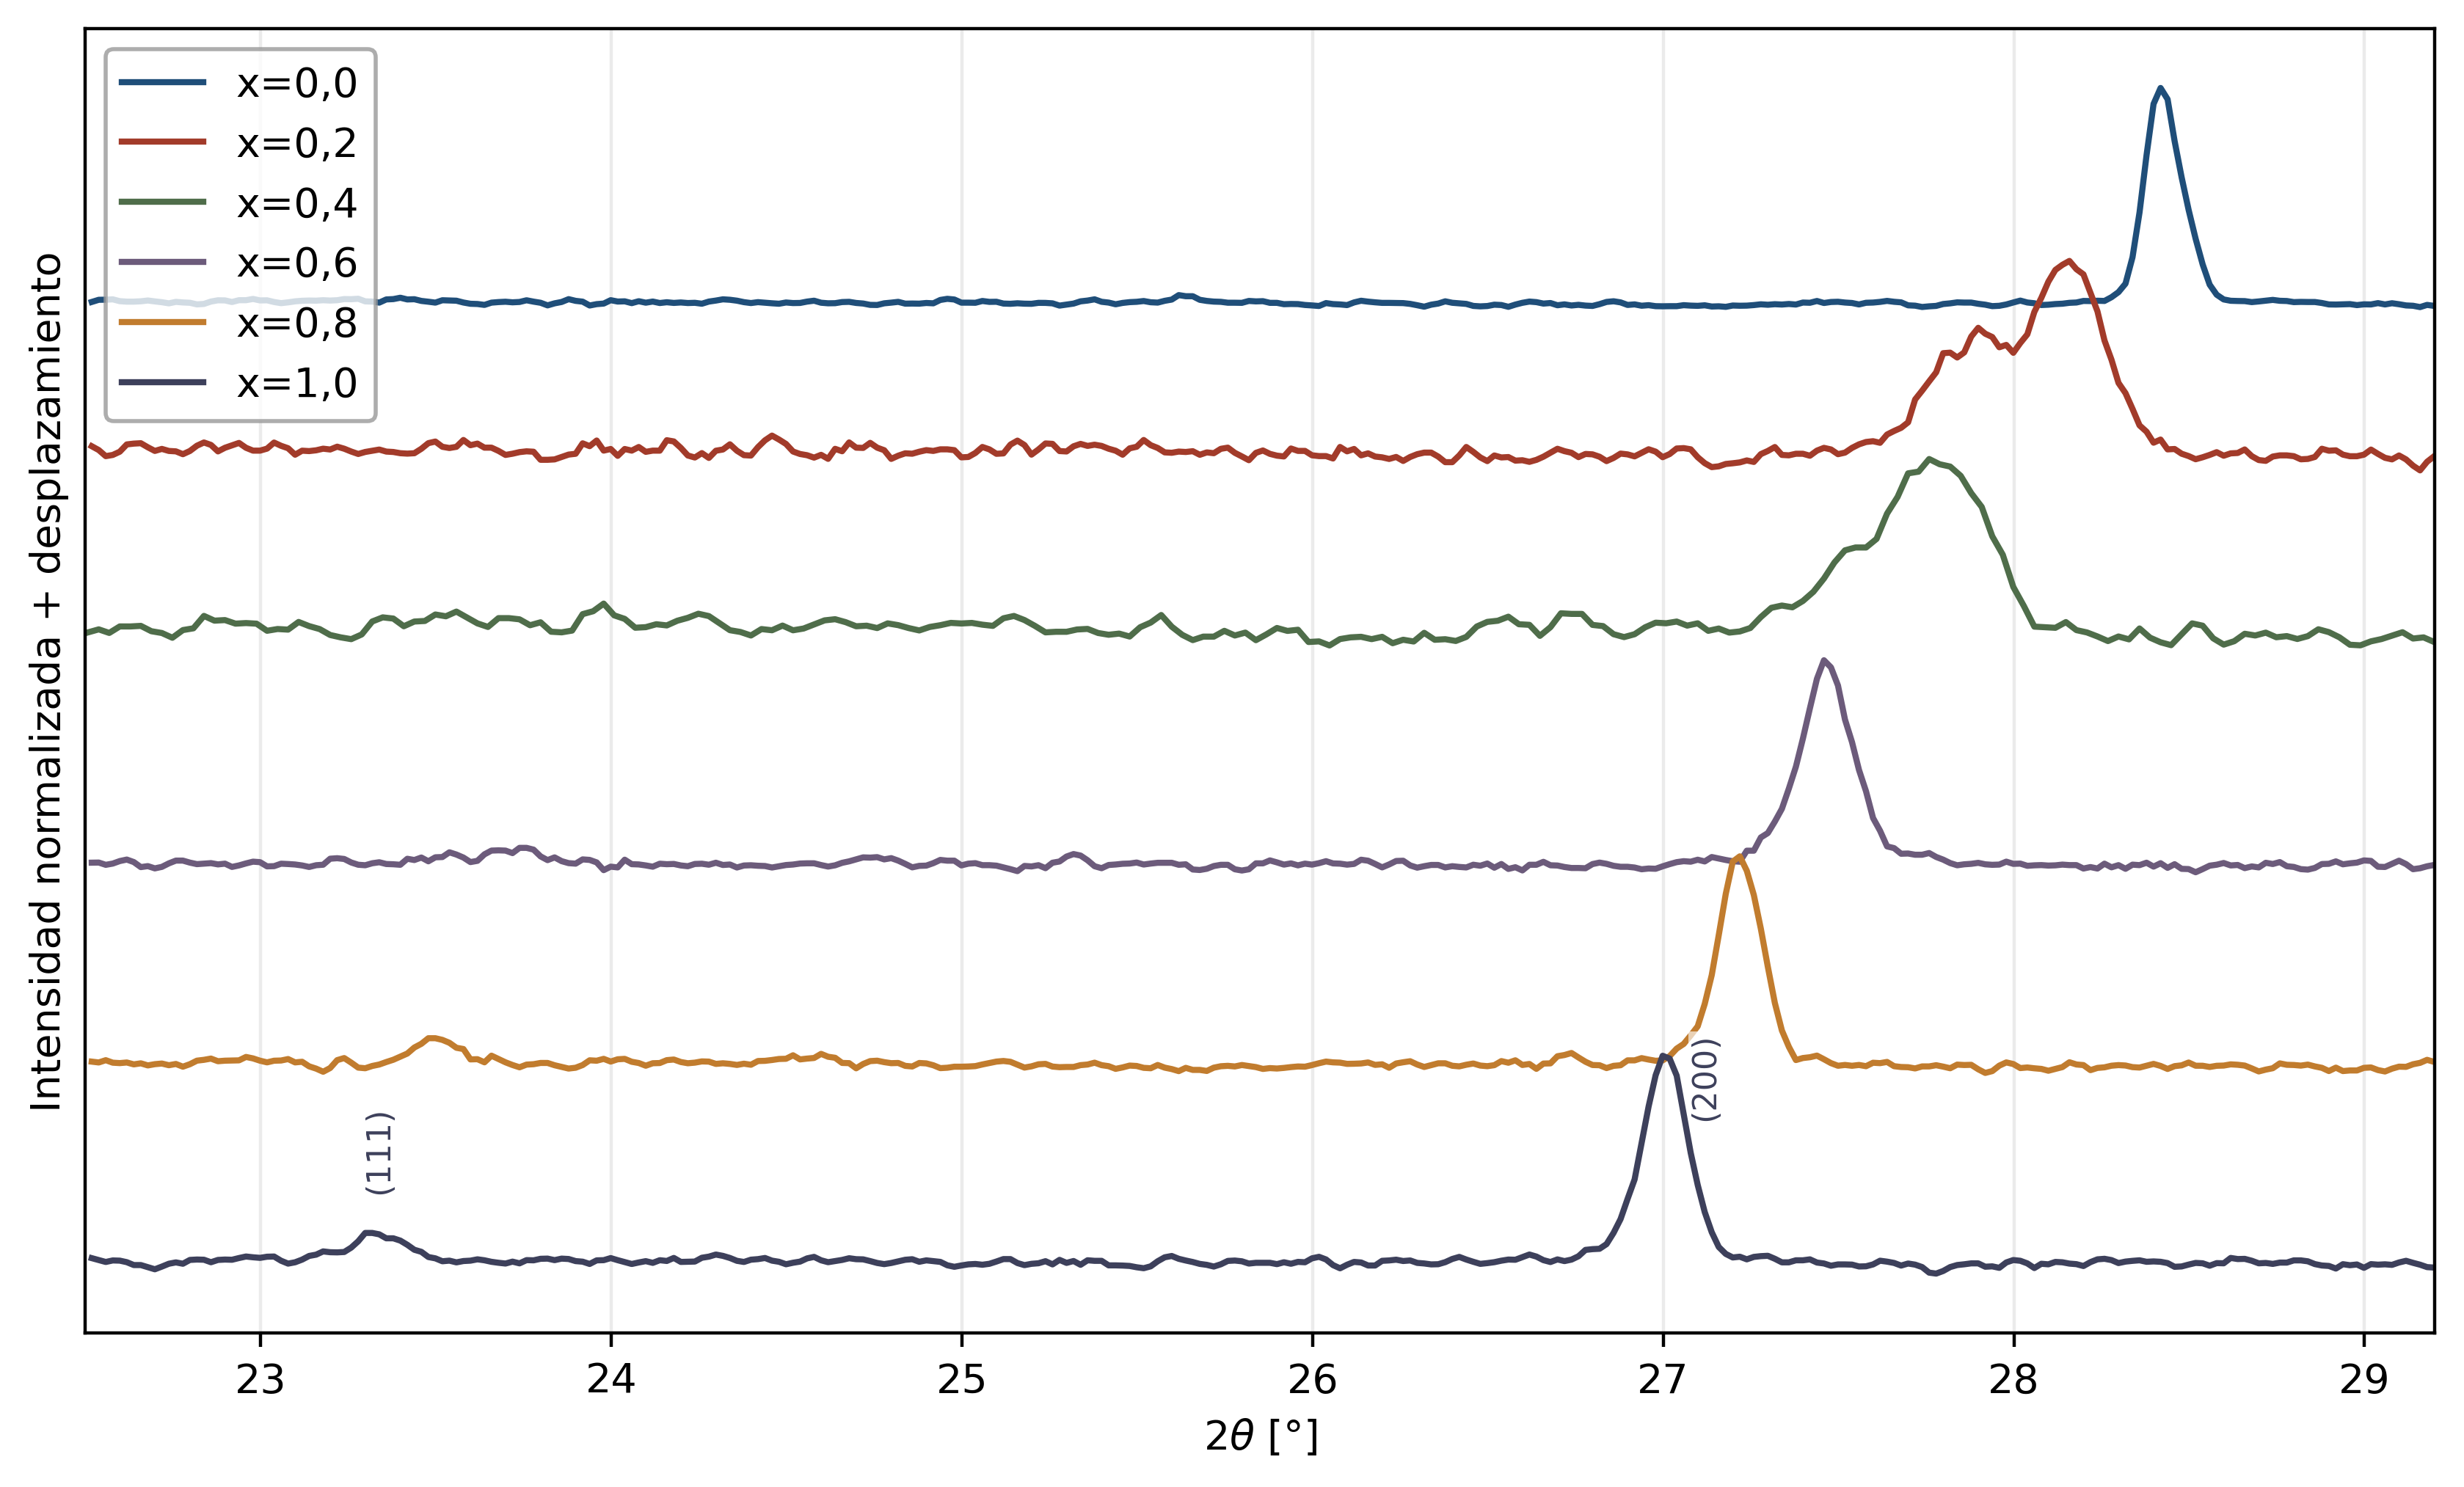
\includegraphics[width=0.5\textwidth]{figuras/zoom_primeros_picos_soluciones.png}
    \caption{Gráfica de los picos de mayor intensidad para cada una de las soluciones analizadas. Donde X representa la fracción molar de KBr en las distintas soluciones.}
    \label{fig:zoom_picos}
\end{figure}
